\documentclass{article}

\usepackage{amsmath, amsthm, amssymb, amsfonts}
\usepackage{thmtools}
\usepackage{graphicx}
\usepackage{setspace}
\usepackage{geometry}
\usepackage{float}
\usepackage{hyperref}
\usepackage[utf8]{inputenc}
\usepackage[english]{babel}
\usepackage{framed}
\usepackage[dvipsnames]{xcolor}
\usepackage{tcolorbox}

%Define the listing package
\usepackage{listings} %code highlighter
\usepackage{color} %use color
\definecolor{mygreen}{rgb}{0,0.6,0}
\definecolor{mygray}{rgb}{0.5,0.5,0.5}
\definecolor{mymauve}{rgb}{0.58,0,0.82}
 
%Customize a bit the look
\lstset{ %
backgroundcolor=\color{white}, % choose the background color; you must add \usepackage{color} or \usepackage{xcolor}
basicstyle=\footnotesize, % the size of the fonts that are used for the code
breakatwhitespace=false, % sets if automatic breaks should only happen at whitespace
breaklines=true, % sets automatic line breaking
captionpos=b, % sets the caption-position to bottom
commentstyle=\color{mygreen}, % comment style
deletekeywords={...}, % if you want to delete keywords from the given language
escapeinside={\%*}{*)}, % if you want to add LaTeX within your code
extendedchars=true, % lets you use non-ASCII characters; for 8-bits encodings only, does not work with UTF-8
frame=single, % adds a frame around the code
keepspaces=true, % keeps spaces in text, useful for keeping indentation of code (possibly needs columns=flexible)
keywordstyle=\color{blue}, % keyword style
% language=Octave, % the language of the code
morekeywords={*,...}, % if you want to add more keywords to the set
numbers=left, % where to put the line-numbers; possible values are (none, left, right)
numbersep=5pt, % how far the line-numbers are from the code
numberstyle=\tiny\color{mygray}, % the style that is used for the line-numbers
rulecolor=\color{black}, % if not set, the frame-color may be changed on line-breaks within not-black text (e.g. comments (green here))
showspaces=false, % show spaces everywhere adding particular underscores; it overrides 'showstringspaces'
showstringspaces=false, % underline spaces within strings only
showtabs=false, % show tabs within strings adding particular underscores
stepnumber=1, % the step between two line-numbers. If it's 1, each line will be numbered
stringstyle=\color{mymauve}, % string literal style
tabsize=2, % sets default tabsize to 2 spaces
title=\lstname % show the filename of files included with \lstinputlisting; also try caption instead of title
}
%END of listing package%
 
\definecolor{darkgray}{rgb}{.4,.4,.4}
\definecolor{purple}{rgb}{0.65, 0.12, 0.82}
 
%define Javascript language
\lstdefinelanguage{JavaScript}{
keywords={typeof, new, true, false, catch, function, return, null, catch, switch, var, if, in, while, do, else, case, break},
keywordstyle=\color{blue}\bfseries,
ndkeywords={class, export, boolean, throw, implements, import, this},
ndkeywordstyle=\color{darkgray}\bfseries,
identifierstyle=\color{black},
sensitive=false,
comment=[l]{//},
morecomment=[s]{/*}{*/},
commentstyle=\color{purple}\ttfamily,
stringstyle=\color{red}\ttfamily,
morestring=[b]',
morestring=[b]"
}
 
\lstset{
language=JavaScript,
extendedchars=true,
basicstyle=\footnotesize\ttfamily,
showstringspaces=false,
showspaces=false,
numbers=left,
numberstyle=\footnotesize,
numbersep=9pt,
tabsize=2,
breaklines=true,
showtabs=false,
captionpos=b
}

\colorlet{LightGray}{White!90!Periwinkle}
\colorlet{LightOrange}{Orange!15}
\colorlet{LightGreen}{Green!15}

\newcommand{\HRule}[1]{\rule{\linewidth}{#1}}

\NewEnviron{NORMAL}{% 
    \scalebox{2}{$\BODY$} 
} 

\declaretheoremstyle[name=Theorem,]{thmsty}
\declaretheorem[style=thmsty,numberwithin=section]{theorem}
\tcolorboxenvironment{theorem}{colback=LightGray}

\declaretheoremstyle[name=Proposition,]{prosty}
\declaretheorem[style=prosty,numberlike=theorem]{proposition}
\tcolorboxenvironment{proposition}{colback=LightOrange}

\declaretheoremstyle[name=Principle,]{prcpsty}
\declaretheorem[style=prcpsty,numberlike=theorem]{principle}
\tcolorboxenvironment{principle}{colback=LightGreen}

\setstretch{1.2}
\geometry{
    textheight=9in,
    textwidth=5.5in,
    top=1in,
    headheight=12pt,
    headsep=25pt,
    footskip=30pt
}

% ------------------------------------------------------------------------------

\begin{document}

% ------------------------------------------------------------------------------
% Cover Page and ToC
% ------------------------------------------------------------------------------

\title{ \normalsize \textsc{}
		\\ [2.0cm]
		\HRule{1.5pt} \\
		\LARGE \textbf{\uppercase{Statistica}
		\HRule{2.0pt} \\ [0.6cm] \LARGE{Corso A} \vspace*{10\baselineskip}}
		}
\date{\text{Ultima Compilazione - }\today}
\author{\textbf{Autore} \\ 
		Giuseppe Acocella \\
		2024/25\\}

\maketitle
\newpage

\tableofcontents

\newpage

\section{Statistica Descrittiva}

Questo ramo della statistica cerca di raccogliere dati per descrivere degli oggetti. Elenchiamo delle definizioni standard:

\begin{enumerate}
    \item \textbf{Popolazione}: Insieme di oggetti da studiare.
    \item \textbf{Carattere}: Caratteristiche degli oggetti della popolazione.
    \begin{enumerate}
        \item Colore di una biglia, altezza di un individuo.
    \end{enumerate}
    Ricordiamo che un carattere può essere sia \textbf{qualitativo} (es. colore) sia \textbf{quantitativo} (es. altezza).
    \item \textbf{Modalità}: Possibili valori che il carattere può assumere.
    \begin{enumerate}
        \item Colore biglia istanziato: rosso, blu. Lancio moneta istanziato: testa/croce.
    \end{enumerate}
    \item \textbf{Campione Statistico (Sample)}: Sottoinsieme della popolazione scelto a rappresentarla.
    \item \textbf{Dati}: Esiti delle misure del carattere sugli individui del campione.
    \begin{enumerate}
        \item Lanci moneta: $T,C,T,T,T,C, \;....$
    \end{enumerate}
    \item \textbf{Taglia Campione}: Numero di elementi nel campione.
\end{enumerate}

\subsection{Frequenze e Campioni}

Abbiamo due tipi di frequenze:

\begin{enumerate}
    \item \textbf{Frequenza Assoluta}: Corrisponde al numero di volte in cui la \textbf{modalità} appare nei \textbf{dati}:
    \[ \#\{\: i \: |\:x_{i} = a \:\} \]
    \item \textbf{Frequenza Relativa}: Corrisponde al numero di volte in cui la \textbf{modalità} appare nei dati fratto il numero dei dati stessi:
    \[ \text{frequenza relativa} = \frac{\text{frequenza assoluta di }a}{\text{taglia campione}} \]
\end{enumerate}

\subsection{Caratteri e Rappresentazioni Grafiche}


La rappresentazione dei dati dipende fortemente dal tipo di \textbf{carattere}:
\vspace*{10px}
\begin{enumerate}
    \item \textbf{Carattere Discreto}: Quantità piccola e finita di modalità assumibili.
    \begin{enumerate}
        \item Lancio di un dado, esiti di un sondaggio.
    \end{enumerate}

\newpage

In questo caso per le rappresentazioni si utilizzano \textbf{diagrammi a barre}.

\begin{figure}[htbp]
    \center
    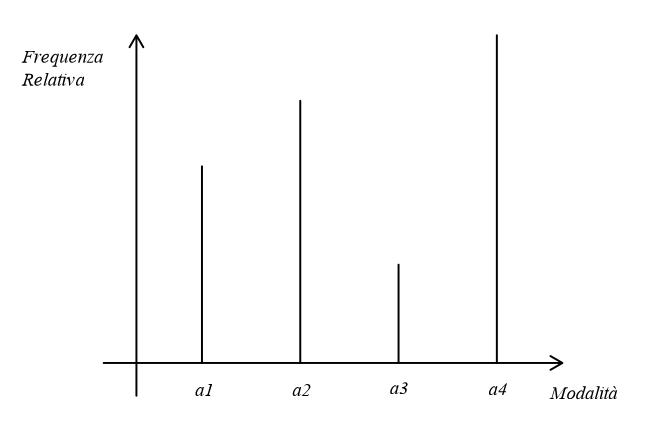
\includegraphics[scale=0.6]{img/diagramma_a_barre.png}
    \caption{Esempio di diagramma a barre.}
\end{figure}

\item \textbf{Carattere Continuo}: Quantità assumibili in un intervallo continuo.
\begin{enumerate}
    \item Altezza della popolazione.
\end{enumerate}

\begin{figure}[htbp]
    \center
    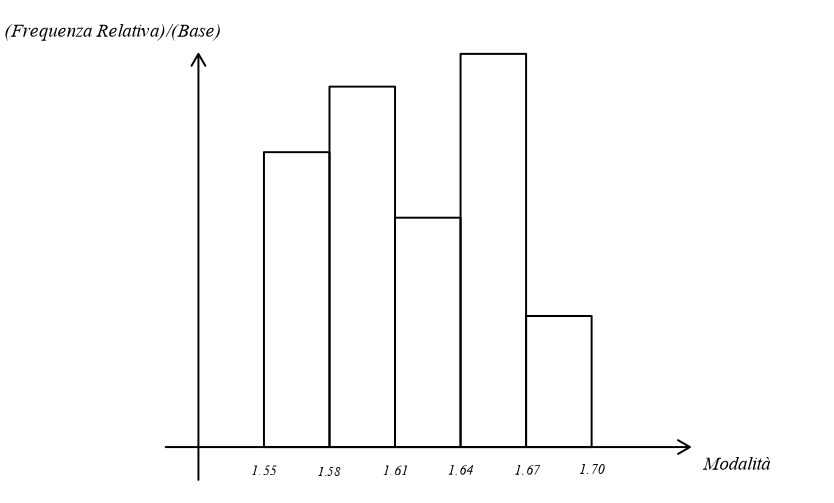
\includegraphics[scale=0.5]{img/istogramma.png}
    \caption{Esempio di istogramma.}
\end{figure}

\vspace*{8px}

La scelta di mettere sull'asse y il rapporto tra freq. relativa e base non è casuale, infatti se scegliessimo intervalli di ampiezza diversa si andrebbe in contro ad un errore di rappresentazione.

\end{enumerate}

\newpage

\subsubsection{Classi di grafici}

Elenchiamo qualche classificazione di rappresentazioni grafiche:

\begin{enumerate}
    \item \textbf{Normale}: Simile ad una campana simmetrica:
    \begin{figure}[htbp]
        \center
        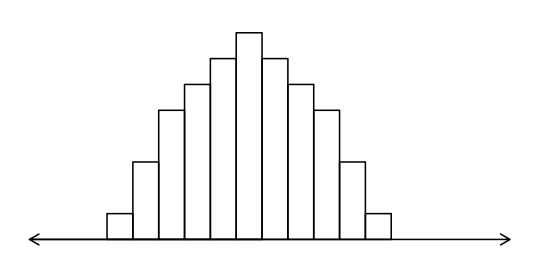
\includegraphics[scale=0.5]{img/normale.png}
    \end{figure}
    \vspace*{8px}

    \item \textbf{Uni/Bi/Tri Modale}: Si concentra attorno ad un numero k di colonne più alte:
    \begin{figure}[htbp]
        \center
        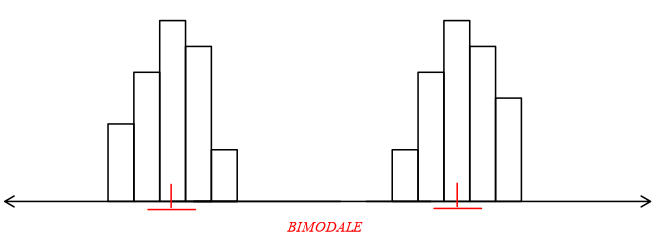
\includegraphics[scale=0.5]{img/modale.png}
    \end{figure}
    \vspace*{8px}

    \begin{enumerate}
        \item \textbf{Modale Asimmetrico Sx/Dx}: Si concentrano attorno ad una colonna più alta in maniera asimmetrica:
        \begin{figure}[H]
  \centering
  \begin{minipage}[b]{0.4\textwidth}
    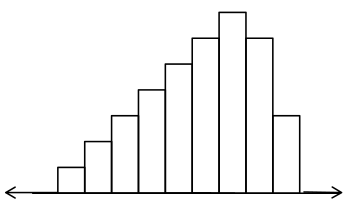
\includegraphics[width=\textwidth]{img/asimmetrico_sx.png}
  \end{minipage}
  \hspace{10px}
  \begin{minipage}[b]{0.4\textwidth}
    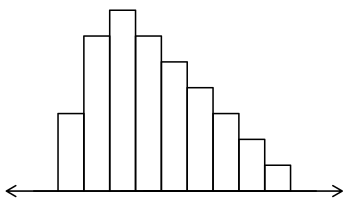
\includegraphics[width=\textwidth]{img/asimmetrico_dx.png}
  \end{minipage}
\end{figure}
    \end{enumerate}
\end{enumerate}

\newpage

\subsection{Indici}

Gli indici statistici sono quantità numeriche che riassumono proprietà significative sulla \textbf{distribuizione dei dati}.

\subsubsection{Indici di Centralità - (Media, Mediana, Moda)}

Descriviamo tre tipi di indici di centralità:

\begin{enumerate}
    \item \textbf{Media Campionaria}: Descriviamo questo indice:
    \[ \overline{x} = \frac{1}{n}\sum_{i=1}^{n} x_{i}\]
    ossia semplicemente la media aritmetica dei dati.
    Un modo \textbf{alternativo} è rappresentarlo così:
    \vspace*{5px}
    \[ \frac{\text{modalita}*\text{frequenza ass. della modalita}}{\text{quantità di dati}} \]
    \vspace*{5px}
    che formalmente si esprime così:
    \[ \overline{x} = \sum_{j=1}^{M}\:a_{j}\:p(a_{j}) \]
    dove $a_{j}$ sta per modalità e $p(a_{j})$ sta per frequenza relativa della modalità.
    \paragraph{Sensibilità ai Valori Estremi} Una delle caratteristiche della media campionaria è quella di essere molto sensibile ai valori estremi del campione.
    \paragraph{Caratteristiche} Riesce a vedere tutti i dati del campione e gode di alcune proprietà matematiche come la linearità.
    \item \textbf{Mediana Campionaria}: Il dato $x_{i}$ sarà \textbf{centrale}, dunque avrà metà dei dati a sinistra e metà a destra. La calcoliamo dunque in due modi:
    \begin{enumerate}
        \item \textbf{Numero dispari di modalità}: Dato centrale.
        \[ \text{mediana} = x(\frac{n+1}{2}) \]
        \item \textbf{Numero pari di modalità}: Media tra i due dati centrali.
        \[ \text{mediana} = \frac{1}{2}(x_{\frac{n}{2}} + x_{\frac{n}{2}+1}) \]
    \end{enumerate}
    \paragraph{Caratteristiche} Più robusta rispetto ai valori estremi.
    \item \textbf{Moda}: Modalità più frequente tra i dati.
\end{enumerate}

\newpage

\subsubsection{Indici di Dispersione - (Varianza, Deviazione Standard)}

Gli indici di dispersione ci permettono di stabilire quanto i valori della distribuzione si allontanino da un valore centrale scelto come riferimento.
Elenchiamoli:

\begin{enumerate}
    \item \textbf{Varianza Campionaria/Empirica}: Permette di 
    \[ \text{CAMPIONARIA:} \:\:\:\: Var(x) = \frac{1}{n-1} \sum^{n}_{i=1}(x_{i}-\overline{x})^{2} \]
    \[ \text{EMPIRICA:} \:\:\:\: Var_{e}(x) = \frac{1}{n} \sum^{n}_{i=1}(x_{i}-\overline{x})^{2} = (\frac{1}{n}\sum^{n}_{i=1}x^{2}_{i}) - \overline{x}^{2}\]
    \vspace*{5px}
    E' possibile calcolare la varianza anche con le frequenze relative:
    \[ Var_{e}(x) = (\:\sum_{j=1}^{M}a^{2}_{j} * p(a_{j})\:) - \overline{x}^{2}\]
    \item \textbf{Scarto Quadratico Medio}: Indice basato sulla varianza.
    \[ \sigma(x) = \sqrt{Var(x}) \]
    \item \textbf{Indice Campionario di Asimmetria}: Un indice che permette di stabilire se una distribuzione sia o meno asimmetrica:
    \[ b = \frac{1}{b^{3}}\frac{1}{n}\sum_{i=1}^{n}(x_{i}-\overline{x})^{3} \]
    \begin{enumerate}
        \item $b>0$: Distribuzione Asimmetrica a destra.
        \item $b<0$: Distribuzione Asimmetrica a sinistra.
    \end{enumerate}
\end{enumerate}

\subsection{Funzione di Ripartizione Empirica (FDR/ECDF)}

Dati $x_{1}, x_{2}, \: ... \:, x_{n}$ dati quantitativi definiamo $F_{e}:\mathbb{R} \xrightarrow{} \mathbb{R}$ data da

\vspace*{10px}

\[ \boxed{F_{e}(t) = \frac{\#\{ \: i \: | \:x_{i} \leq t \: \}}{n}} \]

\subsection{Prova}

\newpage

\end{document}